% !TeX root = ../main.tex

\chapter{基于模型集成的筛选规划算法}\label{chap:mbdp}

基于第~\ref{chap:background}~章中介绍的条件风险价值(CVaR)的思想,本文在强化学习经验回放样本池中加入样本筛选机制的设计,将更低奖励反馈的样本加以更多的学习,而对过高奖励反馈的样本进行适当的筛选和丢弃,确保强化学习算法所学策略能够更稳定地处理高风险状态。

\section{MBDP算法描述与设计}

尽管在CVaR条件风险价值的思路下可以实现鲁棒性的提升,但是显然易见的是,筛选丢弃样本的做法会损失一部分性能。为此,本文提出了基于模型集成的筛选规划算法(Model-Based Dropout Planning,MBDP),在做到提升算法鲁棒性的同时维持原有的算法性能。MBDP算法的整体框架如图\ref{fig:mbdp-structure}~所示,主要流程如算法~\ref{algo:our-method}~所示。

\subsection{环境模型的集成学习与筛选}\label{sec:model-method}

传统的不确定性环境建模和集成方法,虽然已经能够较好地模拟真实复杂环境并且捕捉到环境的不确定性 \cite{duan2007multi,zhang2021mbdp},但并不能很好地控制模拟的精准程度,本论文在不确定性环境建模的基础上,结合传统集成学习的方法,设计了模型的集成和筛选机制。

具体地,首先训练学习一组环境模型集合$\{\mathcal{M}_{\phi_1},\mathcal{M}_{\phi_2},\ldots\}$,集合中每一个环境模型都是一个概率神经网络,其输出$\mu_{\phi_i},\sigma_{\phi_i}$构成高斯分布$\mathcal{N}(\mu_{\phi_i}(s,a),\sigma_{\phi_i}(s,a))$,环境模型对于下一时刻的状态预测则服从该分布,即:
\begin{equation}
    s^\prime \sim \mathcal{M}_{\phi_i}(s,a) = \mathcal{N}(\mu_{\phi_i}(s,a),\sigma_{\phi_i}(s,a)).
\end{equation}
在训练环境模型的同时,根据真实环境中采样得到的真实样本$(S,A)$,可以计算并记录模型的期望偏差:
\begin{equation}
    \mathrm{bias}(\phi_i) = \underset{S,A\sim \pi,\mathcal{P}}{\mathbb{E}}\|\mathcal{M}_{\phi_i}(S,A)-\mathcal{P}(S,A)\|,
\end{equation}
其中$\|\cdot\|$是状态空间$\mathcal{S}$上的范数距离,该式的含义为所训练的环境模型$\mathcal{M}$与真实环境$\mathcal{P}$之间的范数意义距离。在上述模型集合的基础上,首先根据所计算的$\mathrm{bias}(\phi_i)$大小进行升序重排,并设定一个概率参数$\beta\in(0,1]$,筛选出$\mathrm{bias}$在$\beta$分位数以前的模型,保留得到筛选后的模型集合$\mathcal{M}^\beta = \{\mathcal{M}_{\phi_1},\mathcal{M}_{\phi_2},\ldots,\mathcal{M}_{\phi_{N_\beta}}\}$,其中$N_\beta$是前面所描述的升序排序后的集合索引$\left\{1,2,\ldots,N_\beta,\ldots\right\}$中的$\beta$分位数。

需要注意的是,用于集成的不确定性模型集合并不是$\mathrm{bias}$越小越好,过小的$\mathrm{bias}$可能意味着过拟合的环境模型。参数$\beta$的重要用处是可以动态地调整模型集合的整体精确性,它能与下一节将介绍的参数$\alpha$协作调整强化学习的收益性能与鲁棒性。

\subsection{环境模型的数据生成与筛选}\label{sec:rollout-method}

传统的基于模型的强化学习算法在得到环境模型后,往往是以期望收益为目标进行最大化优化,但是期望意义下的最优并不意味着在任意环境下都能有优秀的表现。在实际部署策略的时候,当智能体面对一些受干扰的状态或是信息量不充分的状态时,容易做出一些不合理甚至危险的决策,导致强化学习在实际部署中出现不稳定的情况\cite{zhang2021mbdp}。为了解决这一问题,本论文提出了一种主动关注较坏情况的样本筛选机制,适当延缓强化学习训练速度,提升决策策略的鲁棒性。

具体地,基于上一节得到的$\mathcal{M}^{\beta}$模型集合,在每一步都随机抽取一个模型$\mathcal{M}_{\phi_i}\in\mathcal{M}^\beta$,然后使用该模型进行下一时刻的状态预测,即$s_{t+1}\sim \mathcal{M}_{\phi_t}(s_t,a_t), \phi_t\in\Phi_\beta$,这样的一组状态和动作组成模拟样本$x=\left(s_{t+1},s_t,a_t\right)$,填入缓存池,然后相似地以一个概率参数$\alpha\in(0,1]$进行筛选,从中挑选出反馈奖励值相对较低的样本,得到一个筛选后的$\alpha$分位数样本集合
\begin{equation}
    \mathcal{B}_\alpha^{\pi,\mathcal{M}^\beta}=\left\{x|x\in\mathcal{B}^{\pi,\mathcal{M}^\beta},r(x|s)\leq r_{1-\alpha}(\mathcal{B}^{\pi,\mathcal{M}^\beta}|s), \forall s \in \mathcal{S}\right\},
\end{equation}
其中$\mathcal{B}^{\pi,\mathcal{M}^\beta}=\left\{x|x\triangleq\left(s_{t+1},s_t,a_t\right)\sim\pi,\mathcal{M}^\beta\right\}$, $r_{1-\alpha}(\mathcal{B}^{\pi,\mathcal{M}^\beta}|s)$ 是缓存池 $\mathcal{B}^{\pi,\mathcal{M}^\beta}$的$100\times(1-\alpha)$分位数。

\subsection{算法描述与整体框架}\label{sec:mbdp-description}

\begin{figure}[t]
\centering
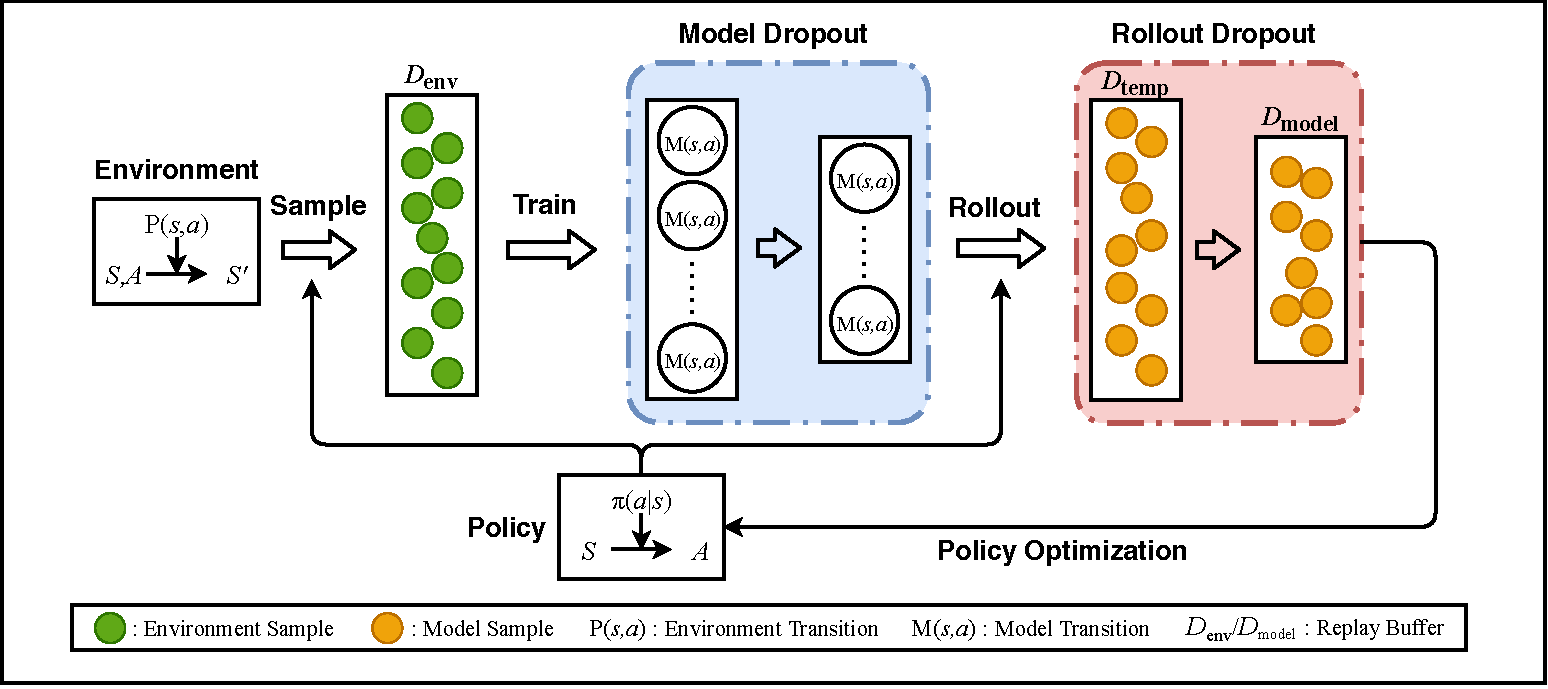
\includegraphics[width=\textwidth]{figures/mbdp.pdf}
\caption{基于模型集成的筛选规划算法示意图}
\label{fig:mbdp-structure}
\end{figure}

\begin{algorithm}[t]
\caption{基于模型集成的筛选规划算法 (\textbf{MBDP})}
\label{algo:our-method}
\begin{algorithmic}
\STATE 初始化超参数、策略 $\pi_\theta$、环境经验回放池 $\mathcal{D}_{\mathrm{env}}$、模型经验回放池 $\mathcal{D}_{\mathrm{model}}$\\
\FOR{$N_\mathrm{epoch}$ 迭代次数}
    \STATE 在环境中使用决策策略 $\pi_\theta$采取行动动作
    \STATE 将样本加入 $\mathcal{D}_{\mathrm{env}}$\\
    \FOR{$N_\mathrm{train}$ 迭代次数}
        \STATE  在收集的数据集$\mathcal{D}_{\mathrm{env}}$上训练概率模型$\mathcal{M}$\\
        \STATE 根据模型偏差$\mathrm{bias}({\phi_i})$构建模型子集 $\mathcal{M}^\beta = \{\mathcal{M}_{\phi_1},\ldots,\mathcal{M}_{\phi_{N_{1-\beta}}}\}$\\
        \FOR{$t=1,2,\ldots ,T$}
            \STATE 从 $\mathcal{M}^\beta$ 中随机抽选模型$\mathcal{M}_{\phi_t}$\\
            \STATE 在模型$\mathcal{M}_{\phi_t}$ 上使用策略$\pi_\theta$,生成样本$x=\left(s_{t+1},s_t,a_t\right)$ \\
            \STATE 将样本填入缓存回放池 $\mathcal{B}^{\pi,\mathcal{M}^\beta}$\\
        \ENDFOR
        \STATE 根据状态$s, \forall s\in\mathcal{S}$分组后计算$100\times(1-\alpha)$分位数,得到 $r_{1-\alpha}(\mathcal{B}^{\pi,\mathcal{M}^\beta}|s)$\\
        \FOR{$x\in \mathcal{B}^{\pi,\mathcal{M}^\beta}$}
            \IF{$r(x)\leq r_{1-\alpha}(\mathcal{B}^{\pi,\mathcal{M}^\beta}|s_t)$}
                \STATE 将 $x$ 填入 $\mathcal{D}_{\mathrm{model}}$
            \ENDIF
        \ENDFOR
    \ENDFOR
    \STATE 在$\mathcal{D}_{\mathrm{model}}$上优化$\pi_\theta$: $\theta\leftarrow \theta - \lambda\nabla_\theta J_\theta(\mathcal{D}_{\mathrm{model}})$
\ENDFOR
\end{algorithmic}
\end{algorithm}


由于在强化学习中模拟误差越小,算法的收敛性能则越好,观察式(\ref{eq:MBDP-bound})中的误差上界$D_{\alpha,\beta}(\mathcal{M})$可知,强化学习的算法性能与参数$\alpha$成反比,与参数$\beta$成正比,又根据~\ref{sec:model-method}~节和~\ref{sec:rollout-method}~节的介绍可知,策略的鲁棒性显然与参数$\alpha$成正比,与参数$\beta$成反比,恰好与前面的作用效果相反。因此,本论文可以动态性地调整参数$\alpha,\beta$来取得算法性能和最终策略鲁棒性之间的平衡,从而得到不同属性的强化学习决策策略:

\begin{itemize}
    \item \textbf{平衡的决策策略}:将参数$\alpha$和$\beta$调整为适中大小的概率值,适用于一般的普通环境;
    \item \textbf{收益性能较高的决策策略}:将参数$\alpha$调整为较小的概率值,$\beta$调整为较大的概率值,适用于相对稳定的环境;
    \item \textbf{鲁棒性较好的决策策略}:将参数$\alpha$调整为较大的概率值,$\beta$调整为较小的概率值,适用于干扰较大的环境。
\end{itemize}

基于~\ref{sec:model-method}~节和~\ref{sec:rollout-method}~节中提出的集成模型筛选模块和模拟数据筛选模块,将其整合加入基于模型的强化学习算法框架,得到改进后的MBDP算法。MBDP算法首先与环境交互产生样本,用于训练概率模型并集成模拟,然后经过集成模型筛选模块生成模拟数据,再由模拟数据筛选模块生成处理后的模拟样本,最终将更新的模拟样本提供给策略优化公式对策略$\pi(a|s)$进行优化,并进行下一轮迭代。

\section{算法理论分析}

记在环境$\mathcal{P}$下,使用策略$\pi$进行交互所得的标准状态价值函数为
\begin{equation}\label{def:eta-s}
    {V}^{\pi,\mathcal{P}}(s) = \underset{\{a_0,s_1,\ldots\} \sim \pi,\mathcal{P}}{\mathbb{E}}\left[\sum_{t=0}^\infty\gamma^t r(s_t,a_t)\mid s_0=s\right].
\end{equation}
为便于分析,使用${V}^{\pi,\mathcal{P}}$表示基于随机初始状态的期望收益:
\begin{equation}\label{def:eta-expectation}
    {V}^{\pi,\mathcal{P}} = \underset{s_0\in\mathcal{S}}{\mathbb{E}} \left[{V}^{\pi,\mathcal{P}}(s_0)\right].
\end{equation}
此时可定义在MBDP方法中缓存池里的模拟样本构成的期望收益为${V}^{\pi,\mathcal{M}_\phi}_\alpha$:
\begin{equation}\label{def:eta-beta}
    {V}^{\pi,\mathcal{M}_\phi}_\alpha=\mathbb{E}\left[{\sum}_{\{s_0,a_0,\ldots\} \sim\mathcal{B}_\alpha^{\pi,\mathcal{M}_\phi}}\left[\gamma^t r(s_t,a_t)\right]\right].
\end{equation}

本文可以证明,加入样本筛选机制后的模拟期望收益,与真实环境中期望收益的差异为一个受参数$\beta$控制的上界,如定理~\ref{the:beta-drop-bound}~所述。

\begin{theorem}\label{the:beta-drop-bound}

记$R_{m}$为奖励函数$r(s,a)$的上确界, 即 $R_{m}=\underset{s\in\mathcal{S},a\in\mathcal{A}}{\sup}r(s,a)$,在环境模型$\mathcal{M}_\phi$上使用样本筛选机制后,所得期望收益与真实环境中期望收益的差异值存在误差上界:
\begin{equation}
    |{V}_\alpha^{\pi, \mathcal{M}_{\phi}} - {V}^{\pi,\mathcal{M}_{\phi}}| \leq \frac{\alpha(1+\alpha)}{(1-\alpha)(1-\gamma)}\mathrm{R_{m}} \triangleq \epsilon_\alpha.
\label{eq:eps-beta}
\end{equation}
\end{theorem}

定理~\ref{the:beta-drop-bound}~的重要意义是,即使筛选掉一批模拟样本,环境模型给出的模拟数据仍具备一定的可靠性,该可靠性由概率参数$\alpha$控制。该定理的证明如下。

\begin{proof}
将期望计算按不同属性的集合进行拆分,得到式(\ref{eq:E=1-a+a}):
% 首先可以证明,对于两个不相交的集合 $A$ 和 $B$($A\cap B=\varnothing$) ,满足下式
% \begin{equation}
%     \mathbb{E}_{A\cup B}\left[X\right] = \mathbb{E}_A\left[X\right]\cdot\mathrm{P}\left(A\right)+\mathbb{E}_B\left[X\right]\cdot\mathrm{P}\left(B\right)
% \end{equation}
% 基于上述性质,可以计算得到
\begin{equation}
\begin{aligned}
    &\mathbb{E}\left[{\sum}_{s_0\in\mathcal{S},\{a_0,s_1,\ldots\} \sim\pi,\mathcal{M}_\phi}\left[\gamma^t r(s_t,a_t)\right]\right] =\\
    &(1-\alpha)\cdot \mathbb{E}\left[{\sum}_{\{s_0,a_0,\ldots\} \sim\mathcal{B}_\alpha^{\pi,\mathcal{M}_\phi}}\left[\gamma^t r(s_t,a_t)\right]\right]+\alpha\cdot\mathbb{E}\left[{\sum}_{\{s_0,a_0,\ldots\} \not\sim\mathcal{B}_\alpha^{\pi,\mathcal{M}_\phi}}\left[\gamma^t r(s_t,a_t)\right]\right].
\end{aligned}\label{eq:E=1-a+a}
\end{equation}
根据式(\ref{def:eta-s}),式(\ref{def:eta-expectation}),式(\ref{def:eta-beta})和式(\ref{eq:E=1-a+a})可推导式(\ref{proof:lem42p1}):
\begin{equation}
\begin{aligned}
{V}^{\pi,\mathcal{M}_\phi}_\alpha&=\mathbb{E}\left[{\sum}_{\{s_0,a_0,\ldots\} \sim\mathcal{B}_\alpha^{\pi,\mathcal{M}_\phi}}\left[\gamma^t r(s_t,a_t)\right]\right]\\
&=\frac{1}{1-\alpha}\mathbb{E}\left[{\sum}_{s_0\in\mathcal{S},\{a_0,s_1,\ldots\} \sim\pi,\mathcal{M}_\phi}\left[\gamma^t r(s_t,a_t)\right]\right]-\\
&\frac{\alpha}{1-\alpha}\mathbb{E}\left[{\sum}_{\{s_0,a_0,\ldots\} \not\sim\mathcal{B}_\alpha^{\pi,\mathcal{M}_\phi}}\left[\gamma^t r(s_t,a_t)\right]\right]\\
&=\frac{1}{1-\alpha}\underset{s\in{\mathcal{S}}}{\mathbb{E}}\left[{V}^{\pi,\mathcal{M}_\phi}(s)\right]-\frac{\alpha}{1-\alpha}\mathbb{E}\left[{\sum}_{\tau \not\sim\mathcal{B}_\alpha^{\pi,\mathcal{M}_\phi}}\left[\gamma^t r(s_t,a_t)\right]\right]\\
&=\frac{1}{1-\alpha}{V}^{\pi,\mathcal{M}_\phi}-\frac{\alpha}{1-\alpha}\mathbb{E}\left[{\sum}_{\tau \not\sim\mathcal{B}_\alpha^{\pi,\mathcal{M}_\phi}}\left[\gamma^t r(s_t,a_t)\right]\right],\label{proof:lem42p1}
\end{aligned}
\end{equation}
其中 $\tau\triangleq\{s_0,a_0,\ldots\}$。根据式 (\ref{def:batch-alpha-beta})中的定义以及  $\mathrm{R}_{m}=\underset{s\in\mathcal{S},a\in\mathcal{A}}{\sup}r(s,a)$,可推导求得关系式(\ref{eq410}):
\begin{equation}\label{eq410}
\begin{aligned}
\mathbb{E}\left[{\sum}_{\tau \not\sim\mathcal{B}_\alpha^{\pi,\mathcal{M}_\phi}}\left[\gamma^t r(s_t,a_t)\right]\right] &\leq\int_{\tau\not\sim{\mathcal{B}_\alpha^{\pi,\mathcal{M}_\phi}}}\left[\sum_{t=0}^\infty\gamma^t \mathrm{R}_m\right]p(\tau)\mathrm{d}\tau\\
&=\left[\sum_{t=0}^\infty\gamma^t\right]\mathrm{R}_m\int_{\tau\not\sim{\mathcal{B}_\alpha^{\pi,\mathcal{M}_\phi}}}p(\tau)\mathrm{d}\tau\\
&= \frac{1}{1-\gamma}\mathrm{R}_m \int_{\tau\not\sim{\mathcal{B}_\alpha^{\pi,\mathcal{M}_\phi}}}p(\tau)\mathrm{d}\tau\\
&=\frac{\alpha}{1-\gamma}\mathrm{R}_m.
\end{aligned}
\end{equation}
与之相似地可以求得式(\ref{eq411}):
\begin{equation}\label{eq411}
\begin{aligned}
V^{\pi,\mathcal{M}_\phi} = \mathbb{E}\left[{\sum}_{\tau \sim\mathcal{B}^{\pi,\mathcal{M}_\phi}}\left[\gamma^t r(s_t,a_t)\right]\right] &\leq\int_{\tau \sim\mathcal{B}^{\pi,\mathcal{M}_\phi}}\left[\sum_{t=0}^\infty\gamma^t \mathrm{R}_m\right]p(\tau)\mathrm{d}\tau\\
&=\left[\sum_{t=0}^\infty\gamma^t\right]\mathrm{R}_m\int_{\tau \sim\mathcal{B}^{\pi,\mathcal{M}_\phi}}p(\tau)\mathrm{d}\tau\\
&= \frac{1}{1-\gamma}\mathrm{R}_m \int_{\tau \sim\mathcal{B}^{\pi,\mathcal{M}_\phi}}p(\tau)\mathrm{d}\tau\\
&=\frac{1}{1-\gamma}\mathrm{R}_m.
\end{aligned}
\end{equation}
根据上述推导得到的两个不等式关系以及式(\ref{proof:lem42p1}),可知满足不等式(\ref{eq:lem42})关系:
\begin{equation}
\begin{aligned}
|{V}_\alpha^{\pi, \mathcal{M}_{\phi}} - {V}^{\pi,\mathcal{M}_{\phi}}| &=  \left|\frac{\alpha}{1-\alpha}V^{\pi,\mathcal{M}_\phi}-\frac{\alpha}{1-\alpha}\mathbb{E}\left[{\sum}_{\tau \not\sim\mathcal{B}_\alpha^{\pi,\mathcal{M}_\phi}}\left[\gamma^t r(s_t,a_t)\right]\right]\right| \\
&\leq\frac{\alpha}{1-\alpha}\left(\left|V^{\pi,\mathcal{M}_\phi}\right|+\left|\mathbb{E}\left[{\sum}_{\tau \not\sim\mathcal{B}_\alpha^{\pi,\mathcal{M}_\phi}}\left[\gamma^t r(s_t,a_t)\right]\right]\right|\right)\\
&\leq \frac{\alpha}{1-\alpha}\left(\frac{1}{1-\gamma}\mathrm{R}_m+\frac{\alpha}{1-\gamma}\mathrm{R}_m\right) \\
&=\frac{\alpha(1+\alpha)}{(1-\alpha)(1-\gamma)}\mathrm{R_{m}}. \label{eq:lem42}
\end{aligned}
\end{equation}
证毕。
\end{proof}

更进一步地,可以证明在同时加入模拟数据筛选模块和集成模型筛选模块后,所得到的策略期望价值仍然与真实环境下的策略收益存在一个可控的误差上界,并且该上界由筛选比例$\alpha$和$\beta$控制。

\begin{theorem}\label{the:MBDP-bound}

设 $K\geq 0$ 是一项常数。 在同时加入模拟数据筛选模块和集成模型筛选模块后所得到的策略期望价值 ${V}_\alpha^{\pi, \mathcal{M}^\beta}$,与真实环境$\mathcal{P}$下所能得到的期望策略价值 ${V}^{\pi, \mathcal{P}}$存在如式(\ref{eq413})所述的误差上界:
\begin{equation}\label{eq413}
\left|{V}_\alpha^{\pi, \mathcal{M}^\beta}-{V}^{\pi, \mathcal{P}}\right|\leq D_{\alpha,\beta}(\mathcal{M}),
\end{equation}
其中
\begin{equation}\label{eq:MBDP-bound}
D_{\alpha,\beta}(\mathcal{M})\triangleq\frac{(1-\beta)\gamma K}{1-\gamma}\epsilon_{\mathcal{M}}+\frac{\alpha(1+\alpha)(1-\beta)}{(1-\alpha)(1-\gamma)}\mathrm{R}_m,
\end{equation}
并且
\begin{equation}\label{def:delta-M}
\epsilon_{\mathcal{M}}\triangleq\underset{\phi\in\Phi}{\mathbb{E}}\left[\underset{s,a\sim \pi,\mathcal{P}}{\mathbb{E}}\left[\left\|\mathcal{M}_\phi(s, a)-\mathcal{P}(s, a)\right\|\right]\right].
\end{equation}

\end{theorem}
为了证明上述定理,首先需要引入两个引理:
\begin{lemma}\label{lem:proof-for-lem41}
给出定义式(\ref{def:G-sa}):
\begin{equation}\label{def:G-sa}
G^{\pi,\mathcal{M}}(s,a)=\underset{\hat{s}'\sim\mathcal{M}(\cdot|s,a)}{\mathbb{E}}{{V}^{\pi,\mathcal{M}}}(\hat{s}') - \underset{s'\sim\mathcal{P}(\cdot|s,a)}{\mathbb{E}}{{V}^{\pi,\mathcal{M}}}(s'),
\end{equation}
对于任意策略 $\pi$ 和任意动态模型 $\mathcal{M},\mathcal{M}'$,存在关系式(\ref{eq417})
\begin{equation}\label{eq417}
{V}^{\pi,\mathcal{M}'} - {V}^{\pi,\mathcal{M}} = \frac{\gamma}{1-\gamma}\underset{S,A\sim\pi,\mathcal{M}}{\mathbb{E}}\left[G^{\pi,\mathcal{M}'}(S,A)\right].
\end{equation}
\end{lemma}

引理~\ref{lem:proof-for-lem41}~改写自Luo等\cite{luo2018algorithmic}在其论文中提出的定理。在该引理的基础上,本文进一步推导出如下的引理~\ref{lem:mb-bound}~。

\begin{lemma}\label{lem:mb-bound}
设基于模型方法所能取得的价值函数 ${V}^{\pi,\mathcal{M}}$ 在状态空间$\mathcal{S}$上是Lipschitz连续的,并设$K$为 Lipschitz常数,。记$\mathcal{P}$表示真实环境的状态转移概率分布,则有如式(\ref{eq418})的不等式关系:
\begin{equation}\label{eq418}
\left|{V}^{\pi, \mathcal{M}}-{V}^{\pi, \mathcal{P}}\right| \leq\frac{\gamma}{1-\gamma}K\cdot\mathrm{bias},
\end{equation}
其中
\begin{equation}
\mathrm{bias} \triangleq \underset{s,a\sim \pi,\mathcal{P}}{\mathbb{E}}\left\|\mathcal{M}(s, a)-\mathcal{P}(s, a)\right\|.
\end{equation}

\label{theo:mb-bound}
\end{lemma}

引理~\ref{lem:mb-bound}~中假设了关于估计模型$\mathcal{M}$的期望收益${V}^{\pi,\mathcal{M}}(s)$ 关于任意范数距离$\|\cdot\|$都是Lipschitz连续的,即满足式(\ref{assum:lip}):
\begin{equation}\label{assum:lip}
    \left|{V}^{\pi,\mathcal{M}}(s)-{V}^{\pi,\mathcal{M}}(s^{\prime})\right| \leq K\left\|s-s^{\prime}\right\|, \forall s, s^{\prime} \in \mathcal{S},
\end{equation}
其中$K\in \mathbb{R}^+$ 是一个Lipschitz常数。该假设的意义是相近的状态应该拥有相似的价值估计,对于绝大多数场景而言,这一假设显然都是成立的。引理~\ref{lem:mb-bound}~的证明如下:

\begin{proof}

根据$G^{\pi,\mathcal{M}}(s,a)$在式(\ref{def:G-sa})中的定义,以及假设 ${V}^{\pi,\mathcal{M}}(s)$ 满足 Lipschitz 连续性(\ref{assum:lip}), 可以得到式(\ref{eq:G-leq}):
\begin{equation}\label{eq:G-leq}
|G^{\pi,\mathcal{M}}(s,a)|\leq K\|\mathcal{M}(s,a)-\mathcal{P}(s,a)\|.
\end{equation}
因此
\begin{equation}
\begin{aligned}
\left|{V}^{\pi, \mathcal{M}}-{V}^{\pi, \mathcal{P}}\right| &= \frac{\gamma}{1-\gamma}\left|\underset{s,a\sim\pi,\mathcal{P}}{\mathbb{E}}\left[G^{\pi,\mathcal{M}}(s,a)\right]\right|\\
&\leq \frac{\gamma}{1-\gamma}\underset{s,a\sim\pi,\mathcal{P}}{\mathbb{E}}\left[\left|G^{\pi,\mathcal{M}}(s,a)\right|\right]\\
&\leq \frac{\gamma}{1-\gamma}\underset{s,a\sim\pi,\mathcal{P}}{\mathbb{E}}K\|\mathcal{M}(s,a)-\mathcal{P}(s,a)\|\\
&= \frac{\gamma}{1-\gamma}K\cdot\underset{s,a\sim\pi,\mathcal{P}}{\mathbb{E}}\|\mathcal{M}(s,a)-\mathcal{P}(s,a)\|\\
&\triangleq \frac{\gamma}{1-\gamma}K\cdot\mathrm{bias}.
\end{aligned}
\end{equation}
证毕。
\end{proof}

定理~\ref{the:MBDP-bound}~的重要意义是,在加入模拟数据筛选模块和集成模型筛选模块后,模型给出的模拟数据与传统的模拟方式相比只存在一个可控的误差上界,对强化学习的训练带来的误差影响并不大,在该可控范围内,如前文对筛选机制的具体描述,本论文能够得到鲁棒性更好的决策策略。

基于前文证明得到的定理~\ref{the:beta-drop-bound}~和引理~\ref{lem:mb-bound}~,可以进一步证明得到定理~\ref{the:MBDP-bound}~,具体证明过程如下。

\begin{proof}

根据定理~\ref{the:beta-drop-bound}~和引理~\ref{lem:mb-bound}~,首先可以证明:
\begin{equation}
\begin{aligned}
\left|{V}_\alpha^{\pi, \mathcal{M}^\beta}-{V}^{\pi, \mathcal{P}}\right|&=\left|\int_{\Phi_\beta}{V}_\alpha^{\pi, \mathcal{M}_{\phi}}p(\phi)\mathrm{d}\phi-{V}^{\pi, \mathcal{P}}\right| \\
&=\left|\int_{\Phi_\beta}\left({V}_\alpha^{\pi, \mathcal{M}_{\phi}}-{V}^{\pi, \mathcal{P}}\right)p(\phi)\mathrm{d}\phi\right| \\
&\leq\int_{\Phi_\beta}\left|{V}_\alpha^{\pi, \mathcal{M}_{\phi}}-{V}^{\pi, \mathcal{P}}\right|p(\phi)\mathrm{d}\phi\\
&\leq\int_{\Phi_\beta}\left(\left|{V}^{\pi, \mathcal{M}_{\phi}}-{V}^{\pi, \mathcal{P}}\right|+\left|{V}_\alpha^{\pi, \mathcal{M}_{\phi}} - {V}^{\pi,\mathcal{M}_{\phi}}\right|\right)p(\phi)\mathrm{d}\phi\\
&= \int_{\Phi_\beta}\left|{V}^{\pi, \mathcal{M}_{\phi}}-{V}^{\pi, \mathcal{P}}\right|p(\phi)\mathrm{d}\phi+\int_{\Phi_\beta}\left|{V}_\alpha^{\pi, \mathcal{M}_{\phi}} - {V}^{\pi,\mathcal{M}_{\phi}}\right|p(\phi)\mathrm{d}\phi. \label{proof:theo43p1}
\end{aligned}
\end{equation}
对于式 (\ref{proof:theo43p1})的第一部分,记
\begin{equation}
\epsilon_{\mathcal{M}}\triangleq\underset{\phi\in\Phi}{\mathbb{E}}\left[\underset{s,a\sim \pi,\mathcal{P}}{\mathbb{E}}\left[\left\|\mathcal{M}_\phi(s, a)-\mathcal{P}(s, a)\right\|\right]\right]
\end{equation}
表示在模型$\mathcal{M}$和环境$\mathcal{P}$之间的一般性偏差。根据引理~\ref{lem:mb-bound}~,可以求得:
\begin{equation}
\begin{aligned}
\int_{\Phi_\beta}\left|{V}^{\pi, \mathcal{M}_{\phi}}-{V}^{\pi, \mathcal{P}}\right|p(\phi)\mathrm{d}\phi &\leq \frac{\gamma K}{1-\gamma}\int_{\Phi_\beta}\underset{s,a\sim\pi,\mathcal{P}}{\mathbb{E}}\left[\left\|\mathcal{M}_\phi(s, a)-\mathcal{P}(s, a)\right\|\right]p(\phi)\mathrm{d}\phi\\
&\leq \frac{\gamma K}{1-\gamma}\left|\epsilon_{\mathcal{M}}\right|\int_{\Phi_\beta}\left|p(\phi)\right|\mathrm{d}\phi\\
&=\frac{(1-\beta)\gamma K}{1-\gamma}\epsilon_{\mathcal{M}}. \label{proof:theo43p2}
\end{aligned}
\end{equation}
对于式(\ref{proof:theo43p1})的第二部分, 根据定理~\ref{the:beta-drop-bound}~可以证明:
\begin{equation}
\begin{aligned}
\int_{\Phi_\beta}\left|{V}_\alpha^{\pi, \mathcal{M}_{\phi}} - {V}^{\pi,\mathcal{M}_{\phi}}\right|p(\phi)\mathrm{d}\phi&\leq \frac{\alpha(1+\alpha)}{(1-\alpha)(1-\gamma)}\mathrm{R}_m\int_{\Phi_\beta}p(\phi)\mathrm{d}\phi\\
&=\frac{\alpha(1+\alpha)(1-\beta)}{(1-\alpha)(1-\gamma)}\mathrm{R}_m. \label{proof:theo43p3}
\end{aligned}
\end{equation}
将上述结果代回式(\ref{proof:theo43p1}),可以得到:
\begin{equation}
\begin{aligned}
\left|{V}_\alpha^{\pi, \mathcal{M}^\beta}-{V}^{\pi, \mathcal{P}}\right| &\leq \int_{\Phi_\beta}\left|{V}^{\pi, \mathcal{M}_{\phi}}-{V}^{\pi, \mathcal{P}}\right|p(\phi)\mathrm{d}\phi+\int_{\Phi_\beta}\left|\epsilon_\alpha\right|p(\phi)\mathrm{d}\phi\\
&\leq \frac{(1-\beta)\gamma K}{1-\gamma}\epsilon_{\mathcal{M}}+\frac{\alpha(1+\alpha)(1-\beta)}{(1-\alpha)(1-\gamma)}\mathrm{R}_m\\
&\triangleq D_{\alpha,\beta}(\mathcal{M}).
\end{aligned}
\end{equation}
证毕。
\end{proof}

根据定理~\ref{the:MBDP-bound}~中的的误差上界$D_{\alpha,\beta}(\mathcal{M})$分析可以得出结论,由于$D_{\alpha,\beta}(\mathcal{M})$与$\alpha$成正比,与$\beta$成反比,易知当$\alpha$增大或$\beta$减小时,该误差上界会被扩大,导致算法训练过程中的准确性下降,使得算法需要更长时间才能收敛,最终致使算法的样本效率降低。反之,若$\alpha$减小或$\beta$增大时,算法的样本效率则能得以提升。由于MBDP算法作为基于模型的强化学习算法,可将其更新规则表示为式(\ref{eq:algo-equation}):
\begin{equation}
    \pi_{k+1}, \mathcal{M}^\beta_{k+1}=\underset{\pi_k, \mathcal{M}_k^\beta}{\arg\max}\left[{V}^{\pi_k, \mathcal{M}_k^\beta}-D_{\alpha,\beta}(\mathcal{M}^\beta_k)\right],
\label{eq:algo-equation}
\end{equation}
在该更新式的表达下,本文给出如下的定理
\begin{theorem}
根据式(\ref{eq:algo-equation}),当每一步所得的策略部署在真实环境$\mathcal{P}$中时,其期望收益将会关于步数呈现单调递增趋势,即:
\begin{equation}
    {V}^{\pi_{k+1}, \mathcal{P}}\geq {V}^{\pi_{k}, \mathcal{P}} + (\epsilon_{k+1} - \epsilon_\alpha) \triangleq {V}^{\pi_{k}, \mathcal{P}} + \eta,
\end{equation}
其中
\begin{equation}
    \epsilon_\alpha \triangleq |{V}_\alpha^{\pi, \mathcal{M}_{\phi}} - {V}^{\pi,\mathcal{M}_{\phi}}|   \leq \frac{\alpha}{1-\gamma}\mathrm{R_{m}}.
\end{equation}
而$\epsilon_{k+1}$表示更新残差,记作:
\begin{equation}
    \epsilon_{k+1} \triangleq {V}^{\pi_{k+1}, \mathcal{P}} - \left[{V}_{\alpha}^{\pi_{k+1}, \mathcal{M}_{k+1}^\beta} - D_{\alpha,\beta}(\mathcal{M}_{k+1}^\beta)\right].
\end{equation}
\label{prop:performance}
\end{theorem}

\begin{proof}

根据定理~\ref{the:MBDP-bound}~, $\left|{V}_\alpha^{\pi, \mathcal{M}^\beta}-{V}^{\pi, \mathcal{P}}\right|\leq D_{\alpha,\beta}(\mathcal{M})$,可得:
\begin{equation}\label{eq:prop44p1}
{V}^{\pi_{k+1}, \mathcal{P}} \geq {V}_{\alpha}^{\pi_{k+1}, \mathcal{M}_{k+1}^\beta}-D_{\alpha,\beta}(\mathcal{M}_{k+1}^\beta).
\end{equation}
由于不等式(\ref{eq:prop44p1})的左边部分 ${V}^{\pi_{k+1}, \mathcal{P}}$ 比右边部分${V}_{\alpha}^{\pi_{k+1}, \mathcal{M}_{k+1}^\beta}-D_{\alpha,\beta}(\mathcal{M}_{k+1}^\beta)$大,可将该不等式改写为一个带有残差项$\epsilon_{k+1}$的等式(\ref{proof:prop44p1}):
\begin{equation}\label{proof:prop44p1}
{V}^{\pi_{k+1}, \mathcal{P}} = {V}_{\alpha}^{\pi_{k+1}, \mathcal{M}_{k+1}^\beta}-D_{\alpha,\beta}(\mathcal{M}_{k+1}^\beta) + \epsilon_{k+1},
\end{equation}
其中
\begin{equation}
\epsilon_{k+1} \triangleq {V}^{\pi_{k+1}, \mathcal{P}} - \left[{V}_{\alpha}^{\pi_{k+1}, \mathcal{M}_{k+1}^\beta} - D_{\alpha,\beta}(\mathcal{M}_{k+1}^\beta)\right].
\end{equation}
根据更新规则式(\ref{eq:algo-equation}),可得:
\begin{equation}\label{proof:prop44p2}
{V}_{\alpha}^{\pi_{k+1}, \mathcal{M}_{k+1}^\beta}-D_{\alpha,\beta}(\mathcal{M}_{k+1}^\beta) \geq {V}^{\pi_k,\mathcal{P}}-D_{\alpha,\beta}(\mathcal{P}).
\end{equation}
由于
\begin{equation}
\begin{aligned}
\epsilon_{\mathcal{P}} &= \underset{\phi\in\Phi}{\mathbb{E}}\left[\underset{s,a\sim \pi,\mathcal{P}}{\mathbb{E}}\left[\left\|\mathcal{P}(s, a)-\mathcal{P}(s, a)\right\|\right]\right]\\
&=\underset{\phi\in\Phi}{\mathbb{E}}\left[0\right] = 0,
\end{aligned}
\end{equation}
可以证明:
\begin{equation}
\begin{aligned}
D_{\alpha,\beta}(\mathcal{P}) &= \frac{(1-\beta)\gamma K}{1-\gamma}\epsilon_{\mathcal{P}}+\frac{\alpha(1+\alpha)(1-\beta)}{(1-\alpha)(1-\gamma)}\mathrm{R}_m\\
&=0+\frac{\alpha(1+\alpha)(1-\beta)}{(1-\alpha)(1-\gamma)}\mathrm{R}_m\\
&=\epsilon_\alpha.
\label{proof:prop44p3}
\end{aligned}
\end{equation}
根据式(\ref{proof:prop44p1}),式(\ref{proof:prop44p2})和式(\ref{proof:prop44p3})可知:
\begin{equation}
{V}^{\pi_{k+1}, \mathcal{P}}\geq {V}^{\pi_{k}, \mathcal{P}} + \left[\epsilon_{k+1} - \epsilon_\alpha\right].
\end{equation}
显然可知,更新残差项$\epsilon_{k+1}$在训练阶段远大于$\epsilon_\alpha$,因此满足 $\left[\epsilon_{k+1} - \epsilon_\alpha\right]\geq 0$,从而${V}^{\pi_{k+1}, \mathcal{P}}\geq{V}^{\pi_{k}, \mathcal{P}}+0$。最终可以得到:

\begin{equation}
{V}^{\pi_{0}, \mathcal{P}} \leq \cdots \leq {V}^{\pi_{k}, \mathcal{P}} \leq {V}^{\pi_{k+1}, \mathcal{P}} \leq \cdots
\end{equation}
证毕。
\end{proof}

上述的分析论证了MBDP算法在样本效率上能够确保策略收益随训练步数单调递增,下面对MBDP算法的鲁棒性进行分析论证。本文将鲁棒性定义为算法在受干扰环境下的期望性能。考虑一个干扰矩阵$\hat{\mathcal{P}}=\mathcal{P}_t \circ \delta_t$,其中$\delta_t\in\mathbb{R}^{\mathcal{S}\times\mathcal{A}\times\mathcal{S}}$为可积概率干扰,“$\circ$”为Hadamard乘积记号。根据式(\ref{eq:def-cvar})中对$\mathrm{CVaR}$的定义,本文提出定理~\ref{the:robustness}~。

\begin{theorem}\label{the:robustness}
给定$\alpha\in(0,1)$以及干扰约束集合:
\begin{equation}\label{eq:supp-perturbation}
    \Delta_\alpha \triangleq \left\{\delta_i\middle\vert\prod_{i=1}^{T}\delta_i(s_i\mid s_{i-1},a_{i-1})\leq \frac{1}{\alpha}, \forall s_i\in\mathcal{S}, a_i\in\mathcal{A}\right\}.
\end{equation}
存在如下关系:
\begin{equation}\label{eq:return-cvar-rob}
    V_\alpha^{\pi,\mathcal{M}} = -\mathrm{CVaR}_\alpha\left(-V^{\pi,\mathcal{M}}\right)=\inf\limits_{\Delta_\alpha}\mathbb{E}_{\hat{\mathcal{P}}}\left[V^{\pi,\mathcal{M}}\right].
\end{equation}
\end{theorem}

\begin{proof}
根据 $\mathrm{CVaR}$ 的定义式(\ref{eq:def-cvar})和 $V_\alpha^{\pi,\mathcal{M}}$的定义式(\ref{def:eta-beta}),将奖励反馈取负值用于表示损失,此时可以证明:
\begin{equation}
\begin{aligned}
\mathrm{CVaR}_\alpha(-V^{\pi,\mathcal{M}}) &= \mathbb{E}\left[-V^{\pi,\mathcal{M}}\mid -V^{\pi,\mathcal{M}} \geq \mathrm{VaR}_\alpha(-V^{\pi,\mathcal{M}})\right]\\
&=\mathbb{E}\left[-{\sum}_{\mathcal{B}^{\pi,\mathcal{M}}}\left[\gamma^t r(s_t,a_t)\right]\mid -{\sum}_{\mathcal{B}^{\pi,\mathcal{M}}}\left[\gamma^t r(s_t,a_t)\right] \geq \mathrm{VaR}_\alpha(-V^{\pi,\mathcal{M}})\right]\\
&=-\mathbb{E}\left[{\sum}_{\mathcal{B}^{\pi,\mathcal{M}}}\left[\gamma^t r(s_t,a_t)\right]\mid {\sum}_{\mathcal{B}^{\pi,\mathcal{M}}}\left[\gamma^t r(s_t,a_t)\right] \leq -\mathrm{VaR}_\alpha(-V^{\pi,\mathcal{M}})\right].
\end{aligned}
\end{equation}
显然,上式中的条件 ${\sum}_{\mathcal{B}^{\pi,\mathcal{M}}}\left[\gamma^t r(s_t,a_t)\right] \leq -\mathrm{VaR}_\alpha(-V^{\pi,\mathcal{M}})$ 符合式(\ref{def:batch-alpha-beta})的定义,即:
\begin{equation}\label{def:batch-alpha-beta}
    \mathcal{B}_\alpha^{\pi,\mathcal{M}^\beta}=\left\{x|x\in\mathcal{B}^{\pi,\mathcal{M}^\beta},r(x|s)\leq r_{1-\alpha}(\mathcal{B}^{\pi,\mathcal{M}^\beta}|s), \forall s \in \mathcal{S}\right\},
\end{equation}
因此,定理~\ref{the:robustness}~的第一个等式得证,即:
\begin{equation}
-\mathrm{CVaR}_\alpha(-V^{\pi,\mathcal{M}}) = \mathbb{E}\left[{\sum}_{\mathcal{B}_\alpha^{\pi,\mathcal{M}}}\left[\gamma^t r(s_t,a_t)\right]\right] = V_\alpha^{\pi,\mathcal{M}}.
\end{equation}
考虑到$\mathbb{E}_{\hat{\mathcal{P}}}[-V^{\pi,\mathcal{M}}]$,根据$\hat{\mathcal{P}}$的定义可知:
\begin{equation}
\begin{aligned}
    \mathbb{E}_{\hat{\mathcal{P}}}[V^{\pi,\mathcal{M}}] &= -\mathbb{E}_{\hat{\mathcal{P}}}[-V^{\pi,\mathcal{M}}]\\
    &= -\sum_{(s_0,\ldots,s_T)\in\mathcal{S}^{T+1}}\mathcal{P}_0(s_0)\delta_0(s_0)\prod_{t=1}^{T}\mathcal{P}_t(s_t\mid s_{t-1})\delta_t(s_t\mid s_{t-1})\cdot (-V^{\pi,\mathcal{M}})\\
    &= \sum_{(s_0,\ldots,s_T)\in\mathcal{S}^{T+1}}\mathcal{P}(s_0,\ldots,s_T)\delta_0(s_0)\prod_{t=1}^{T}\delta_t(x_t\mid x_{t-1})\cdot V^{\pi,\mathcal{M}}\\
    &\triangleq \sum_{(s_0,\ldots,s_T)\in\mathcal{S}^{T+1}}\mathcal{P}(s_0,\ldots,s_T)\delta(s_0,\ldots,s_T)\cdot V^{\pi,\mathcal{M}}.
\end{aligned}
\end{equation}
由于$\delta$ 为环境中的随机干扰,显然可知:
\begin{equation}\label{eq:delta-exp}
    \mathbb{E}\left[\delta(s_0,\ldots,s_T)\right] = \sum_{(s_0,\ldots,s_T)\in\mathcal{S}^{T+1}}\mathcal{P}(s_0,\ldots,s_T)\delta(s_0,\ldots,s_T) = 1.
\end{equation}
根据$\Delta_\alpha$ 的定义式(\ref{eq:supp-perturbation}),(\ref{eq:delta-exp})和CVaR的表达性定理\cite{chow2015risk},可以证明定理~\ref{the:robustness}~的第二个等式:
\begin{equation}
\begin{aligned}
    \inf\limits_{\Delta_\alpha}\mathbb{E}_{\hat{\mathcal{P}}}[V^{\pi,\mathcal{M}}] &= \inf\limits_{\delta(s_0,\ldots,s_T)\leq\frac{1}{\alpha}}\sum_{(s_0,\ldots,s_T)\in\mathcal{S}^{T+1}}\mathcal{P}(s_0,\ldots,s_T)\delta(s_0,\ldots,s_T)\cdot V^{\pi,\mathcal{M}}\\
    &=-\mathrm{CVaR}_\alpha(-V^{\pi,\mathcal{M}}).
\end{aligned}
\label{proof:cvar-eq}
\end{equation}
证毕。
\end{proof}

\section{Mujoco环境实验设计与分析}

为了能够进一步验证MBDP算法的实际效果,本文在第~\ref{chap:dper}~章中介绍的强化学习经典测试环境Mujoco仿真程序内进行验证实验。本次实验所使用的代码运行在一台56核CPU、8卡GPU服务器上,具体设备配置如表~\ref{tab:computing-resources}~所示。每项任务在计算机上的计算时间如表~\ref{tab:run-time}~所示。实验所使用的参数如表~\ref{tab:hyperparameters}~所示进行设定。为了证明MBDP方法中上述所加入的模拟数据筛选模块和模型集成筛选模块作为改进方案的可行性,以及验证改进效果,本次实验主要目标为通过实验验证以下问题:

\begin{itemize}
    \item 改进后的算法在强化学习的标准测试任务上相比最新的算法提升如何?
    \item 是否能达到~\ref{sec:rollout-method}~节中所描述的,可通过动态调整参数$\alpha,\beta$来取得不同决策策略的效果?
\end{itemize}

\begin{table}[hbp]
\centering
\caption{MBDP算法验证实验所使用的计算资源}
\begin{tabular}{ccc}
\toprule
CPU                      & GPU                         & RAM   \\
\midrule
Intel E5-2680@2.4GHz (56 Cores) & Tesla P40 (24GB) $\times$ 8 & 256GB\\
\bottomrule
\end{tabular}
\label{tab:computing-resources}
\end{table}

\begin{table}[hbp]
\centering
\caption{MBDP算法在Mujoco环境单次实验在各环境上的计算时间}
\begin{tabular}{ccccc}
\toprule
Environment Name  & Hopper      & Walker2d    & HalfCheetah & Ant         \\
\midrule
Time & $\approx 10$ hours & $\approx 20$ hours & $\approx 32$ hours & $\approx 48$ hours \\
\bottomrule
\end{tabular}
\label{tab:run-time}
\end{table}

在四组不同的Mujoco任务上,与最新的MBPO \cite{janner2019trust}算法、STEVE \cite{buckman2018sample}算法、SLBO \cite{Luo2019AlgorithmicGuarantees}算法以及无模型的SAC \cite{haarnoja2018soft}算法进行对比实验。在本课题的算法中,使用了参数$\alpha=0.2, \beta=0.2$。对比实验结果如图~\ref{fig:performance}~所示,其中横轴为训练的步数,纵轴为相应步数对应的平均收益,每隔1000步统计一次当前累积收益并绘制在图中。实线表示不同随机种子实验(共5组随机数种子)的均值结果,阴影区域则表示这些实验的方差。SAC算法作为一种无模型强化学习算法,其收敛速度相对其他基线算法较慢,因此只在图中画出部分训练曲线图,其最终收敛值通过虚线标注出来。根据实验结果可以看出,基于模型集成的筛选规划算法在四种不同的任务环境中,均有着超越现有算法的表现。

\begin{figure}[ht]
  \centering
  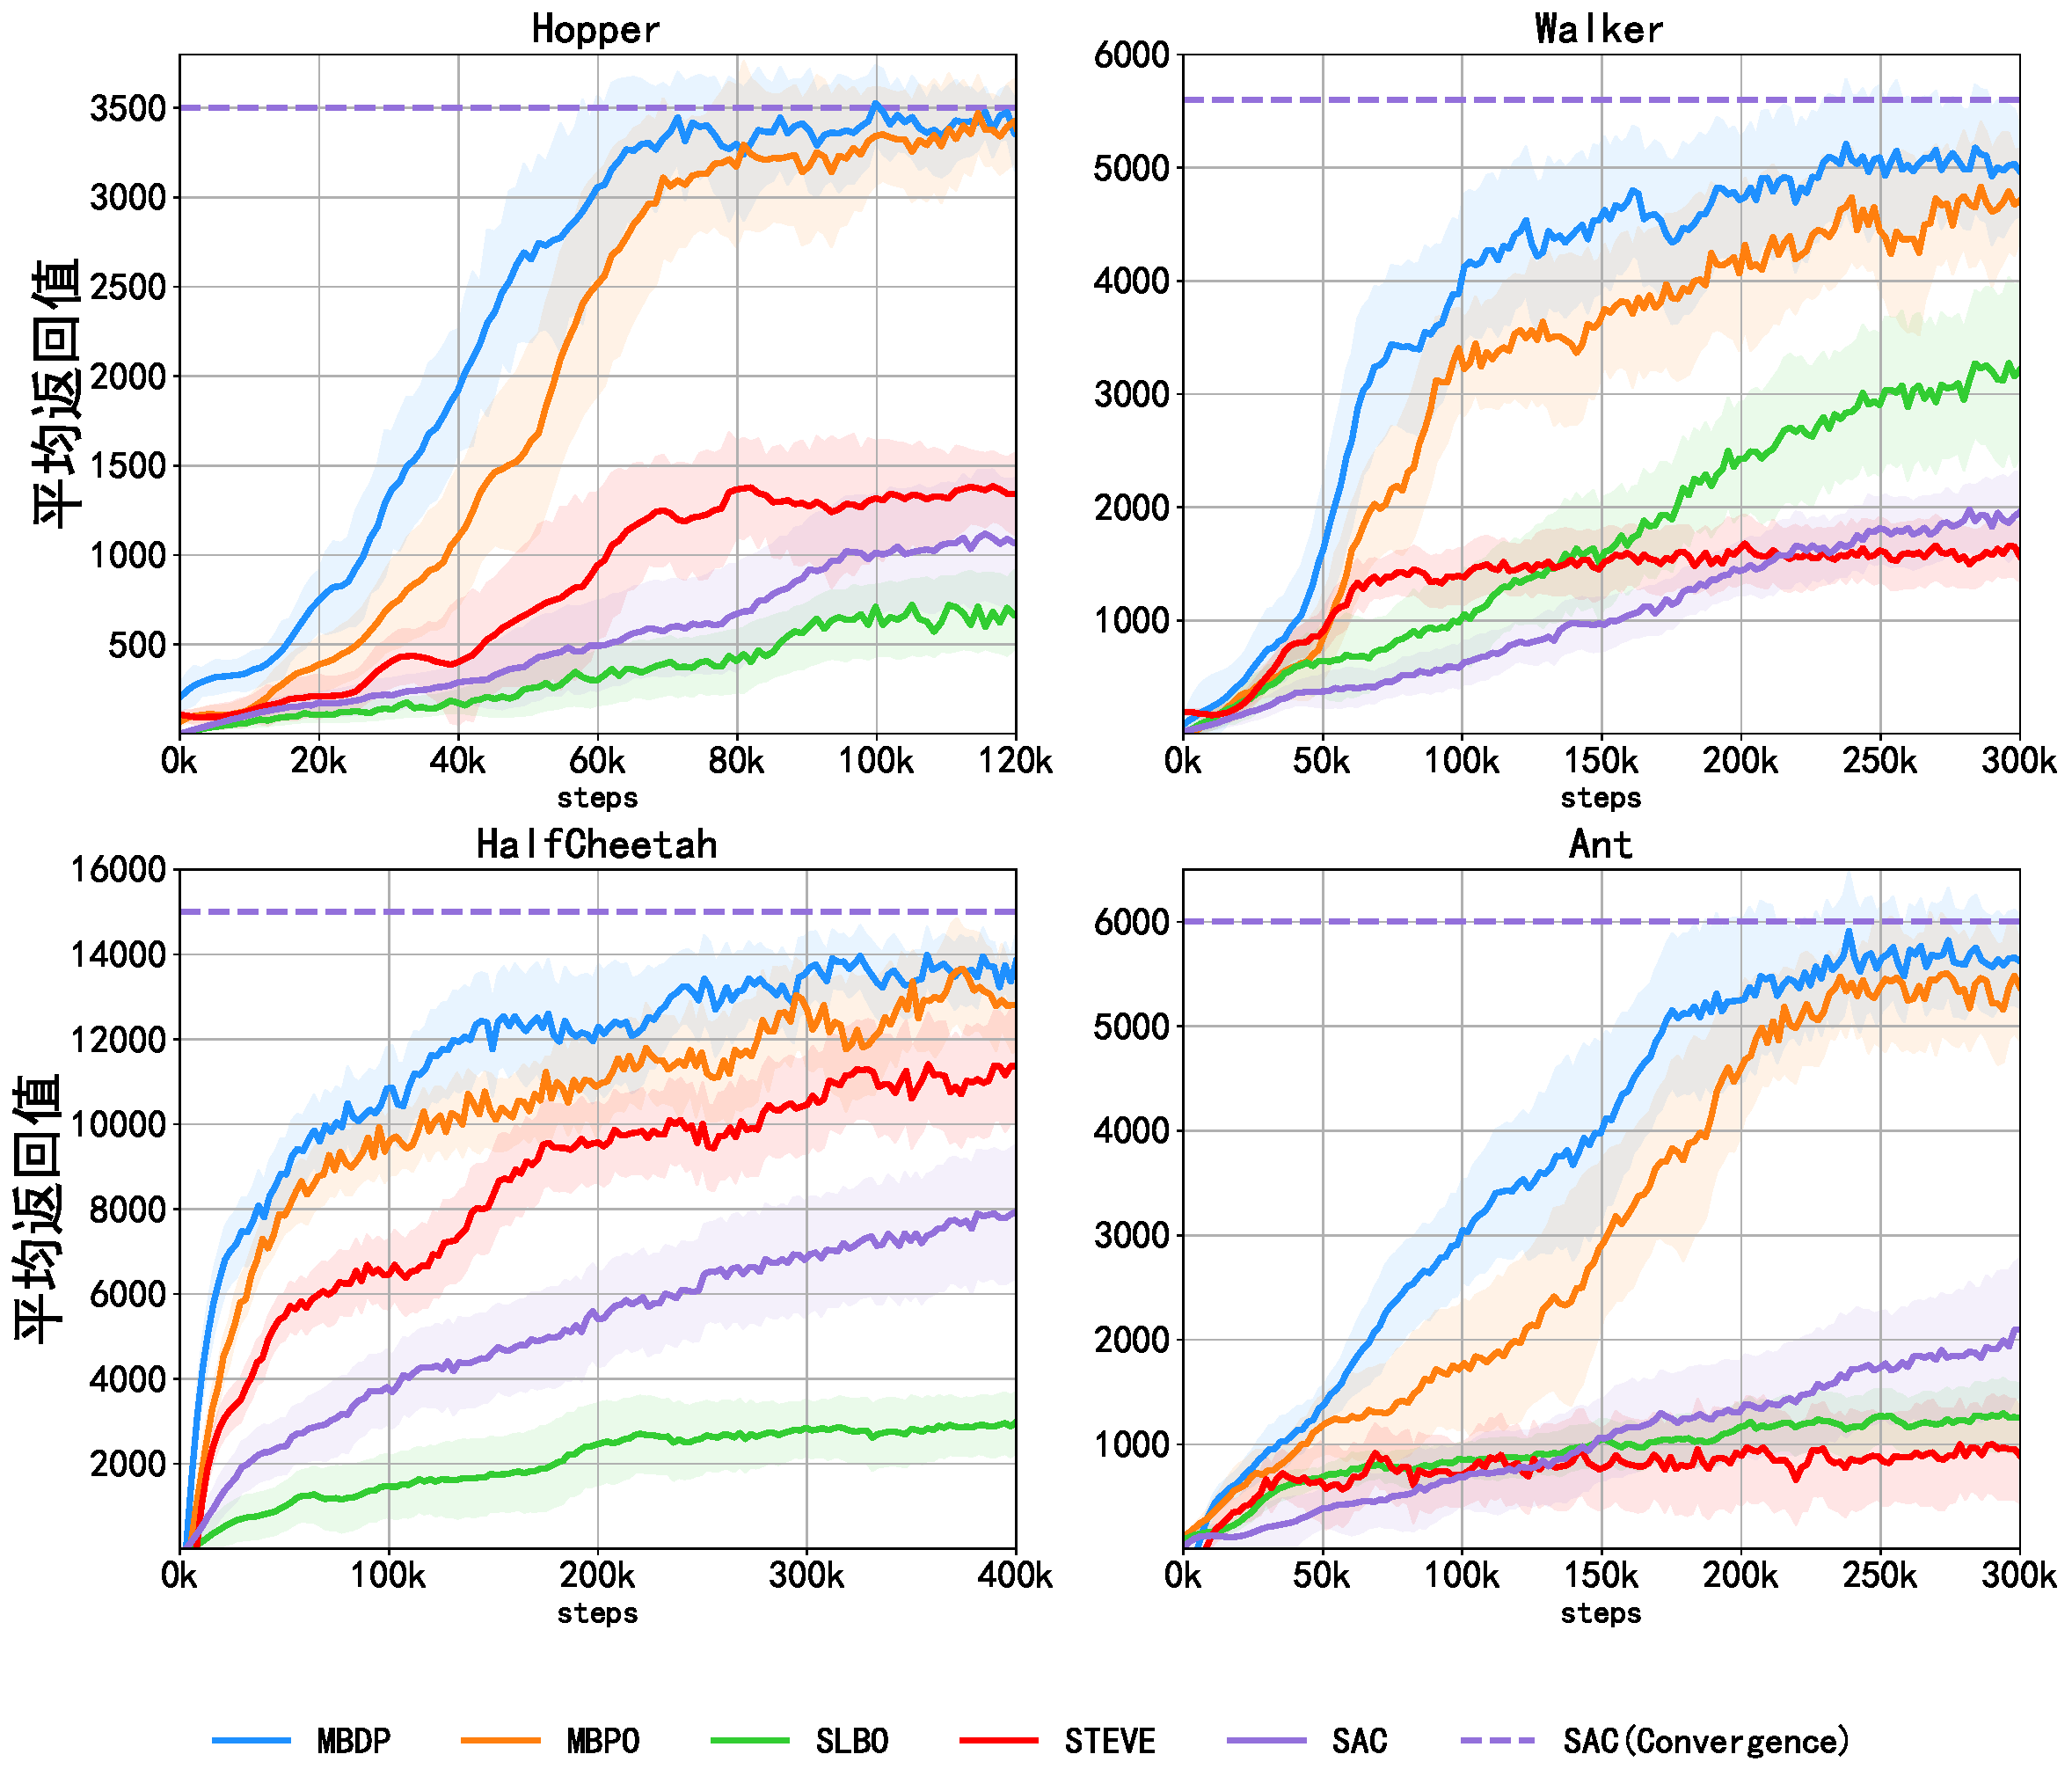
\includegraphics[width=\textwidth]{figures/performance.pdf}
  \caption{MBDP算法与基线算法在不同任务下的训练曲线图}
  \label{fig:performance}
\end{figure}

为了验证MBDP算法对鲁棒性的提升效果,本文对实验环境加入了不同程度的干扰。具体地,在Hopper和HalfCheetah两个任务环境下,将物体的质量和摩擦系数均加以数值区间为$[0.5,1.5]$的干扰,同时以MBPO算法作为对照标准进行对比实验。在每种干扰条件下均进行验证实验,Hopper任务中每组实验训练$3\times 10^5$轮,HalfCheetah任务中每组任务训练$6\times 10^5$轮,实验结果以热力图的形式绘制成图~\ref{fig:robustness-heatmap}~,其中每一个方格表示一组干扰系数下训练相应轮数后的收益值。热力图中的颜色越接近红色代表该环境下的返回值越高,反之颜色越接近蓝色代表返回值越低。在该实验中,共设立了四种不同参数对应的算法,分别是$\alpha=0$,$ \beta=0$的无筛选算法、$\alpha=0.2$,$\beta=0$的$\alpha$-筛选算法、$\alpha=0$,$\beta=0.2$的$\beta$-筛选算法以及$\alpha=0.2$,$\beta=0.2$的同时筛选算法。

\begin{figure}[ht]
  \centering
  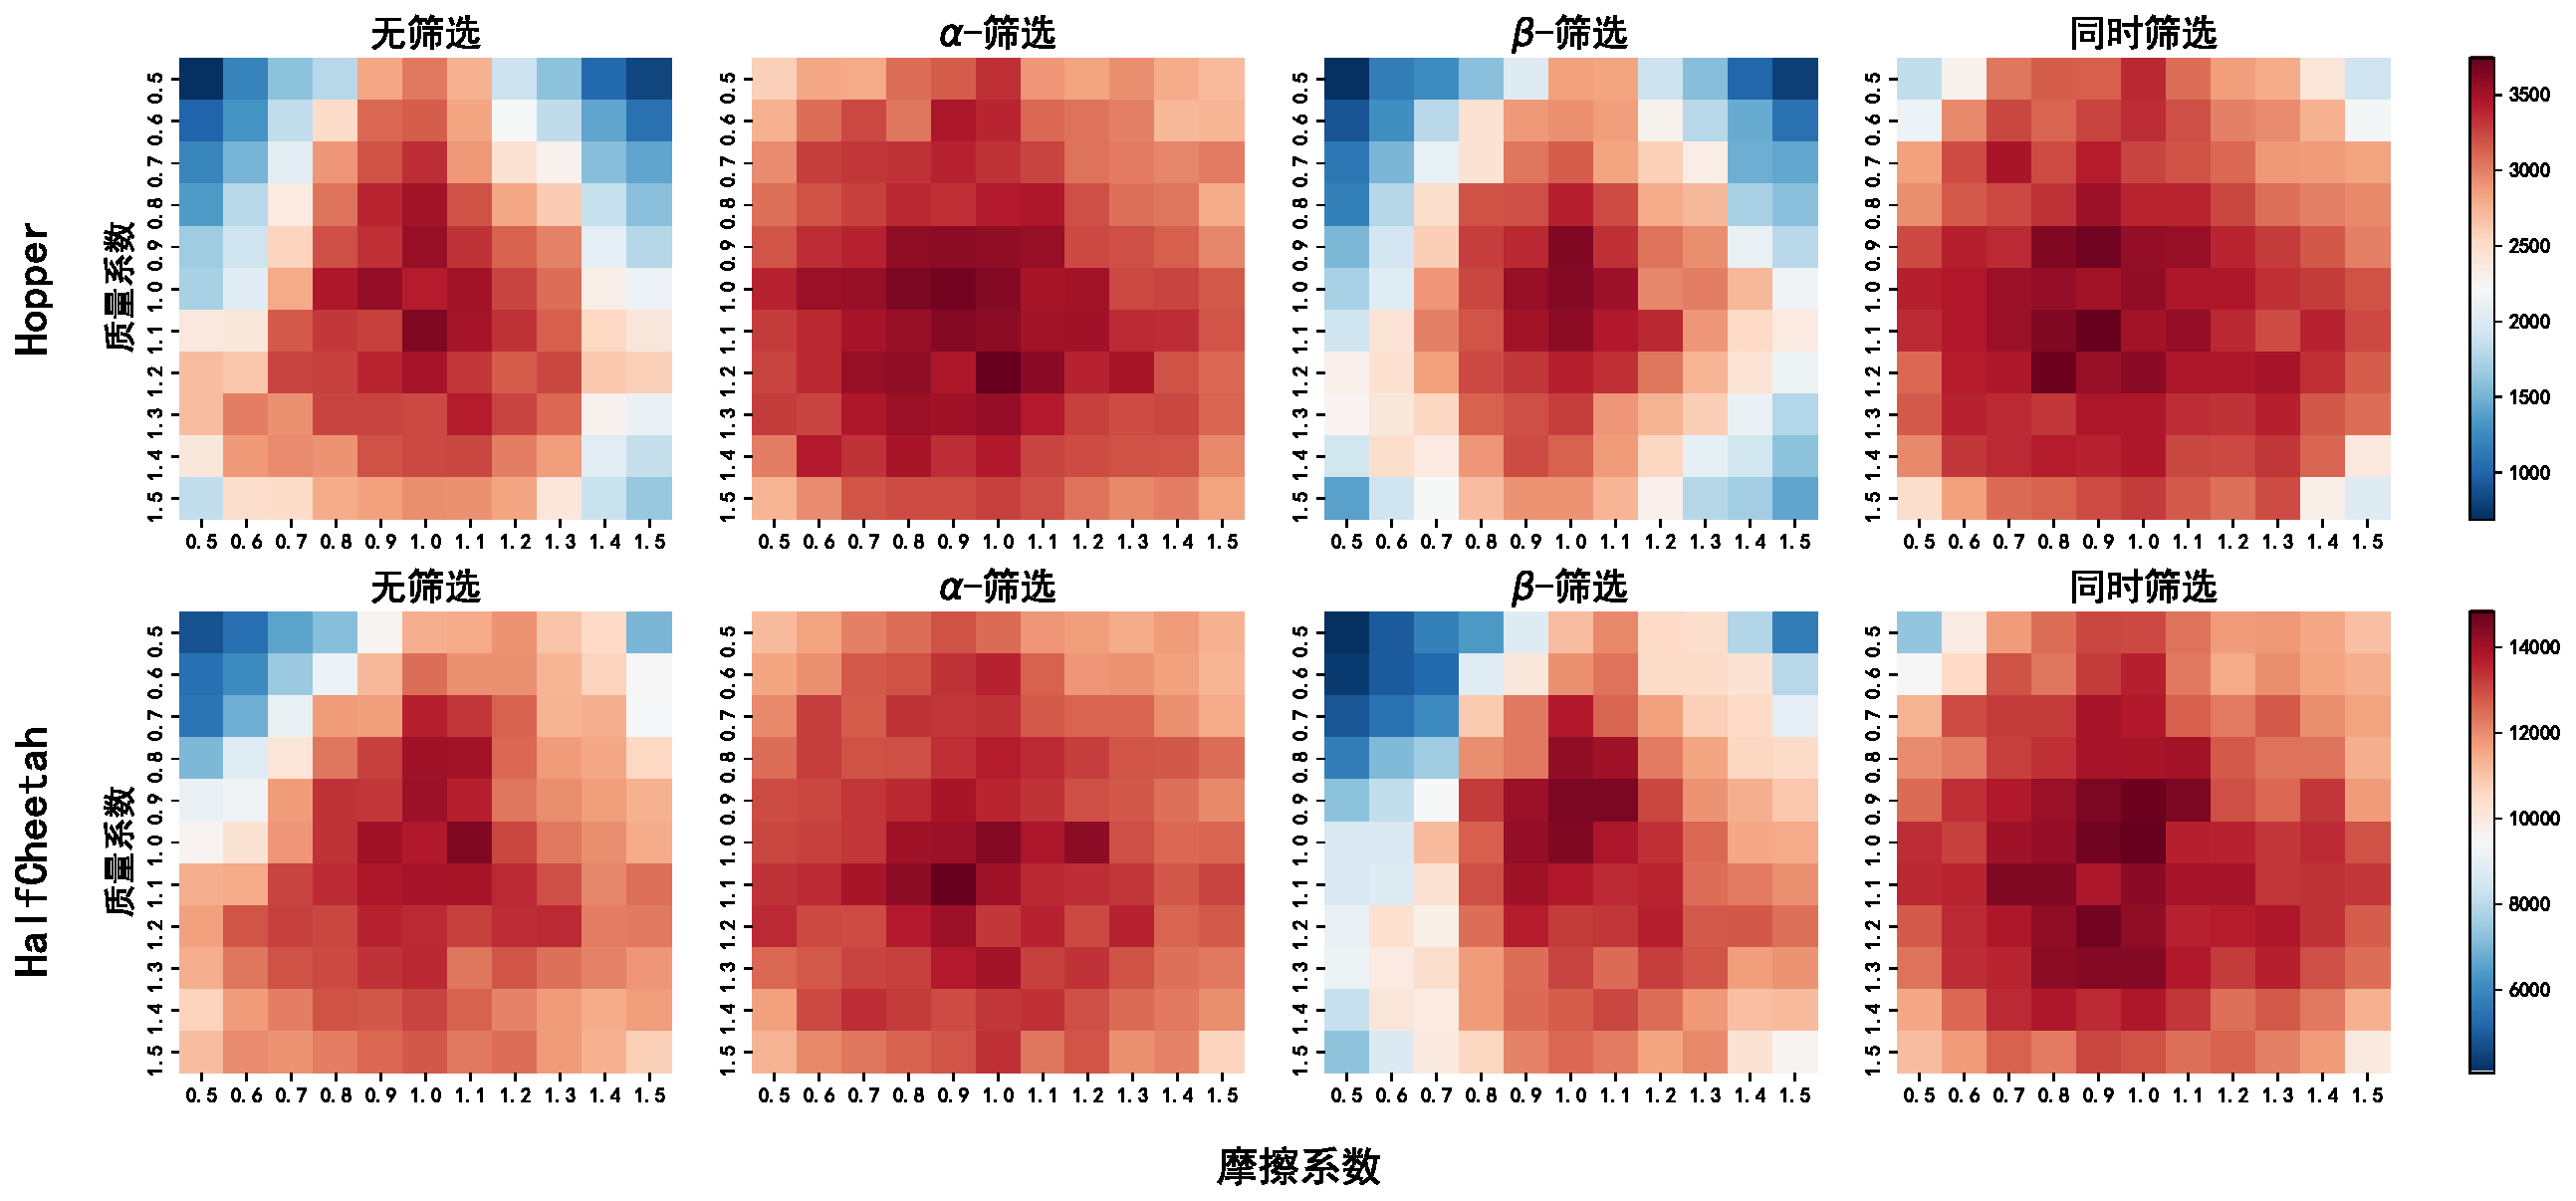
\includegraphics[width=\textwidth]{figures/robustness-heatmap.pdf}
  \caption{MBDP算法鲁棒性对比实验}
  \label{fig:robustness-heatmap}
\end{figure}

\begin{table}[ht]
\centering
\caption{MBDP算法验证实验所使用的参数设定}
\begin{tabular}{ccccccccc}
\toprule
  \begin{tabular}[c]{@{}c@{}}环境\end{tabular} &
  \begin{tabular}[c]{@{}c@{}}训练步数\end{tabular} &
  \begin{tabular}[c]{@{}c@{}}缓存大小\end{tabular} &
  \begin{tabular}[c]{@{}c@{}}策略更新\\步数\end{tabular} &
  \begin{tabular}[c]{@{}c@{}}模型更新\\步数\end{tabular} &
  $\alpha$ &
  $\beta$ &
  $\gamma$ &
  \begin{tabular}[c]{@{}c@{}}网络结构\end{tabular} \\
\midrule
Hopper      & 120000 & $10^5$ & 20 & 250 & 0.2 & 0.2 & 0.99 & \begin{tabular}[c]{@{}c@{}}MLP \\ ($4\times 200$)\end{tabular} \\
Walker    & 300000 & $10^5$ & 20 & 250 & 0.2 & 0.2 & 0.99 & \begin{tabular}[c]{@{}c@{}}MLP \\ ($4\times 200$)\end{tabular} \\
Cheetah & 400000 & $10^5$ & 40 & 250 & 0.2 & 0.2 & 0.99 & \begin{tabular}[c]{@{}c@{}}MLP \\ ($4\times 200$)\end{tabular} \\
Ant         & 300000 & $10^5$ & 20 & 250 & 0.2 & 0.2 & 0.99 & \begin{tabular}[c]{@{}c@{}}MLP \\ ($4\times 200$)
\end{tabular} \\
\bottomrule
\end{tabular}
\label{tab:hyperparameters}
\end{table}

显然可知,如果算法在整个热力图上的性能表现越一致,则说明该算法抗干扰能力更好,鲁棒性更高,反之若在热力图上的性能表现差异越大,则说明该算法更容易受环境干扰影响,鲁棒性更低。观察实验结果中的热力图可知,仅使用模拟数据筛选模块的$\alpha$-筛选算法有着最好的鲁棒性提升,仅使用集成模型筛选模块的$\beta$-筛选算法则会带来鲁棒性下降的负面影响。而当将两种模块结合时,算法仍能维持较好的鲁棒性。这一实验验证了模拟数据筛选模块能够有效提升算法鲁棒性的结论,同时也证明了集成模型筛选模块和模拟数据筛选模块相结合后仍能有正向的鲁棒性提升效果。

为了进一步验证参数$\alpha,\beta$和样本效率与鲁棒性的关系和敏感度,本文设计Hopper和HalfCheetah环境下的参数实验,实验分为两组:

\begin{itemize}
    \item 固定参数$\beta=0.2$,将参数$\alpha$在区间$[0,0.5]$中由小到大进行调整
    \item 固定参数$\alpha=0.2$,将参数$\beta$在区间$[0,0.5]$中由小到大进行调整
\end{itemize}

参数实验的结果如图~\ref{fig:hyper-performance}~所示。图中的第一行为Hopper环境下的实验结果,第二行为HalfCheetah环境下的实验结果。第1、2列为干扰环境实验组的实验结果,在干扰环境实验组中,本文针对每一组摩擦系数和质量系数构建了4种不同的干扰组合,具体地,将质量系数分别设为0.8和1.2,将摩擦系数分别设为0.8和1.2,总共组成$2\times 2=4$种干扰环境。在4个不同的干扰环境下分别进行策略学习,最终所能得到的平均返回值代表算法在受干扰环境中的综合评价指标,该指标越高,说明相应的参数$\alpha,\beta$能使得算法拥有更好的抗干扰性,也即鲁棒性。为了公平比较,本文在Hopper环境下统一训练120000步,在HalfCheetah环境下统一训练400000步。第3、4列为算法在标准环境(摩擦系数和质量系数均为1.0)下所能取得的返回值。同样的,本文在Hopper环境下统一训练120000步,在HalfCheetah环境下统一训练400000步。该项指标可用于评估不同参数下算法的样本利用效率。为了消除随机性的影响,每组实验均由10次随机种子实验组成,并将10次结果统计为箱线图。

\begin{figure}[ht]
  \centering
  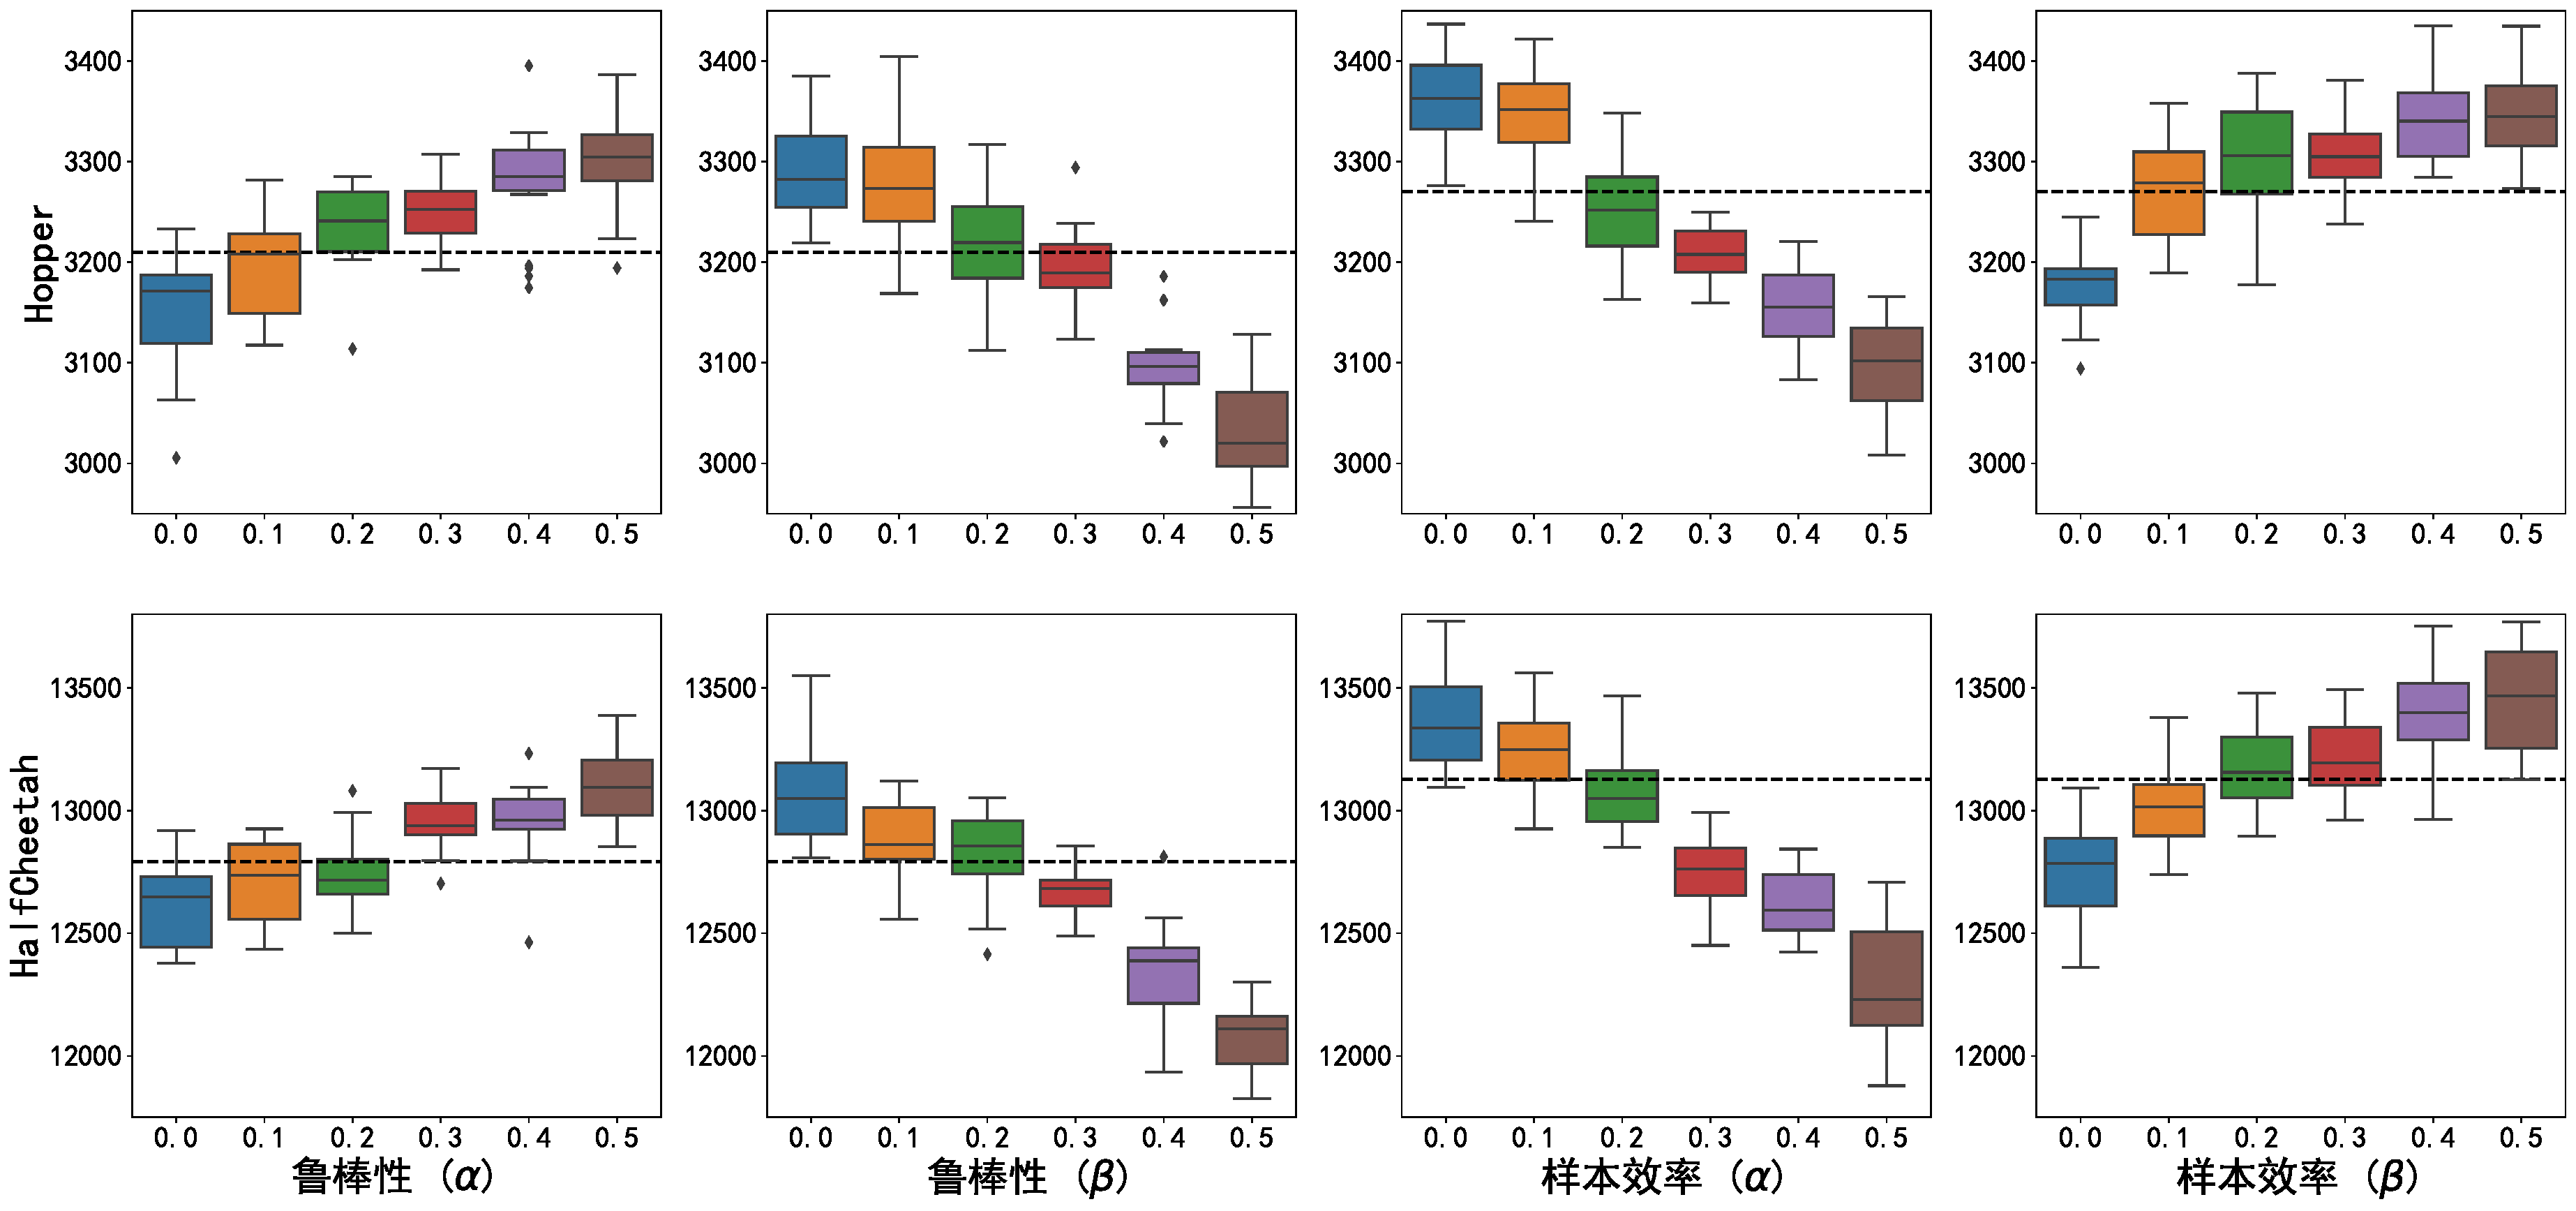
\includegraphics[width=\textwidth]{figures/hyper-performance.pdf}
  \caption{MBDP算法参数敏感性实验}
  \label{fig:hyper-performance}
\end{figure}

观察实验结果,显然可以得出结论,样本利用效率与参数$\alpha$呈现负相关趋势,与参数$\beta$呈现正相关趋势;鲁棒性与参数$\alpha$呈现正相关趋势,与参数$\beta$呈现负相关趋势。这也验证了~\ref{sec:mbdp-description}~节中所提出的MBDP算法与样本利用效率和鲁棒性的关系。此外,本文在实验结果图中用水平虚线画出了不使用任何筛选模块的基线算法($\alpha=\beta=0$)性能,可以看出当$\alpha\in[0.1,0.2]$,$\beta\in[0.1,0.2]$时,MBDP算法能同时得到样本利用效率和鲁棒性的提升。

\section{本章小结}

本章主要介绍了针对强化学习的策略安全性问题提出的基于模型集成的筛选规划算法(Model-Based Dropout Planning,MBDP)。本工作提出了集成模型筛选模块和模拟数据筛选模块,它们共同组合构成了MBDP算法。其中集成模型筛选模块在模型集成方法的基础上,通过计算集成模型中单个模型的预测精确度,对所有模型进行排序,然后按精确度从大到小进行优先级筛选,以少量鲁棒性下降的代价换取模型集成整体精确性的提升,从而实现对算法整体起到样本利用效率的提升;而模拟数据模块则是在基于模型的强化学习方法的基础框架下,对状态转移模型所生成的模拟样本计算收益反馈值,然后排序并按收益值从小到大进行优先级筛选,以少量样本效率下降的代价换取对风险状态的关注程度,提升了策略的稳定性,从而对算法整体起到鲁棒性的提升。集成模型筛选模块和模拟数据筛选模块在对抗的作用下起到了兼顾样本效率提升和鲁棒性提升的平衡效果,其所学习得到的决策策略在保障样本效率的前提下,通过更优秀的鲁棒性来实现决策策略安全性的提升。在本章中,还通过详细的理论分析过程论证了集成模型筛选模块在样本利用效率上的提升效果和模拟数据筛选模块在鲁棒性上的提升效果。并进一步通过模拟仿真实验验证了上述结论。